%==============================================================================
% presentation.tex
%==============================================================================


%==============================================================================
% Configuration
%==============================================================================

% Internationalisation
\usepackage[utf8]{inputenc}
\usepackage[T1]{fontenc}
% \usepackage[ngerman]{babel}

% Different packages
\usepackage{url}
\usepackage{color,listings,paralist}
\usepackage{enumerate}
\usepackage{tabularx}
\usepackage{alltt}

% Use default Acrobat reader fonts
\usepackage{mathpazo}

% Use CM fonts (increases document size)
\usepackage{ae}

% Use images
\usepackage{graphicx}

% Configure beamer
\usetheme[secheader]{Ikhono}
\usefonttheme[onlylarge]{structurebold}
\setbeamertemplate{navigation symbols}{}

% Variables
\providecommand{\Title}{Parallel Programming}
\providecommand{\Subtitle}{Recitation Session 4}
\providecommand{\Author}{Thomas Weibel <weibelt@ethz.ch>}
\providecommand{\Institute}{Laboratory for Software Technology, \\
  Swiss Federal Institute of Technology Z\"urich}
\providecommand{\Date}{March 25, 2010}

% PDF settings
\hypersetup{
  pdftitle={\Title, \Subtitle},
  pdfauthor={\Author},
  pdfsubject={\Institute},
  pdfkeywords={parallel programming} 
}

% Titlepage
\title{\Title}
\subtitle{\Subtitle}
\author{\Author}
\institute{\Institute}
\date{\Date}

% Listings
\lstdefinestyle{Default}{
  language=Java,
  tabsize=2,
  mathescape=true,
  inputencoding=utf8,
  showstringspaces=false,
  fontadjust=true,
  basicstyle=\ttfamily,
  keywordstyle=\color{blue}\bfseries,
  morecomment=[s][\color{blue}]{/*+}{*/},
  morecomment=[s][\color{red}]{/*-}{*/}
}
\lstset{style=Default}


%==============================================================================
% Document
%==============================================================================

\begin{document}


% Titlepage
\begin{frame}[plain]
  \titlepage
\end{frame}


\section*{Introduction}

\begin{frame}{Executive Summary}
  \begin{itemize}
  \item Write parallel MergeSort together
  \item Parallel MergeSort performance
  \item Classroom exercise: Parallel Matrix multiplication
  \end{itemize}
\end{frame}


\section{Parallel MergeSort}

\begin{frame}{Outline}
  \tableofcontents[current]
\end{frame}

\begin{frame}{Questions}
  \begin{itemize}
  \item Is the parallel version faster?
  \item How many threads give the best performance?
  \item What is the influence of the CPU model/CPU frequency?
  \end{itemize}

  \vspace{\stretch{1}}

  \begin{center}
    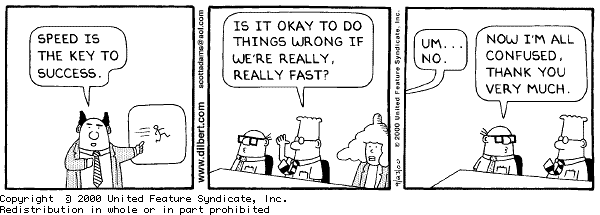
\includegraphics[scale=0.35]{figures/dilbert-1}
  \end{center}
\end{frame}

\begin{frame}[fragile]{Parallel MergeSort}
\begin{lstlisting}
void mergesort (int start, int end) {
  if (end - start >= 1) {
    int middle = (start + end) / 2;
    mergesort(start, middle);
    mergesort(middle+1, end);
    merge(start, middle, middle+1, end);
  }
}
\end{lstlisting}
\end{frame}

\begin{frame}[fragile]{Recursive Thread Creation}
\begin{lstlisting}
void mergesort (int start, int end) {
  if (end - start >= 1) {
    int middle = (start + end) / 2;

    // thread 1 executes the first mergesort
    mergesort(start, middle);

    // thread 2 executes the second mergesort
    mergesort(middle+1, end);

    // join, remaining thread executes merge
    merge(start, middle, middle+1, end);
  }
}
\end{lstlisting}
\end{frame}

\begin{frame}{Example: Graph with 4 Threads}
  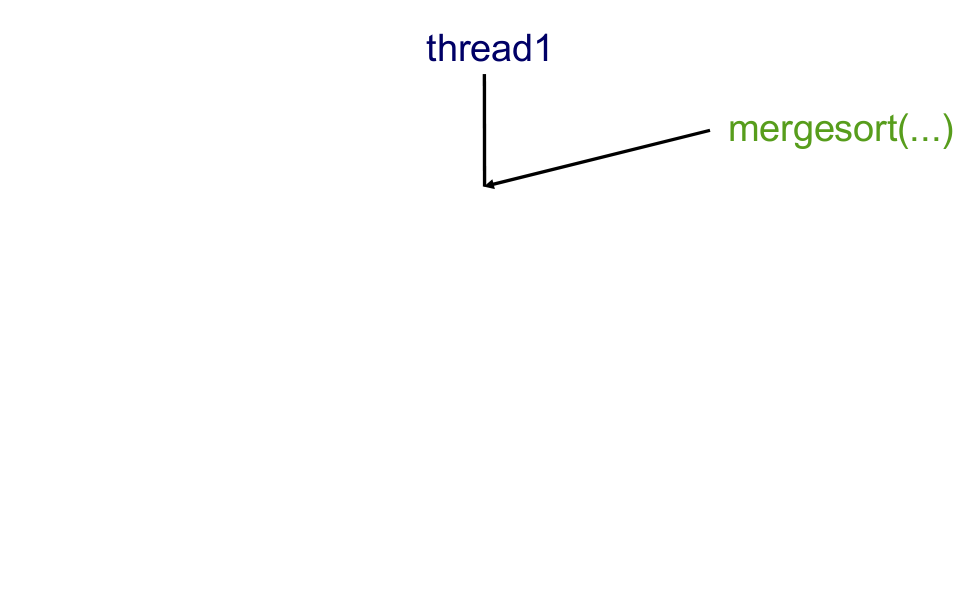
\includegraphics[width=\textwidth]{figures/thread-1}
\end{frame}

\begin{frame}{Example: Graph with 4 Threads}
  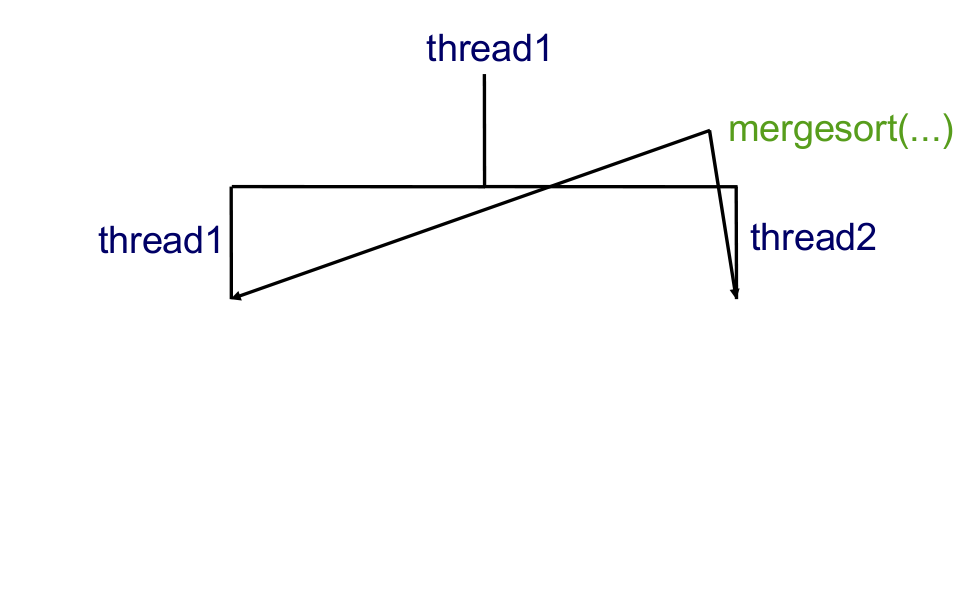
\includegraphics[width=\textwidth]{figures/thread-2}
\end{frame}

\begin{frame}{Example: Graph with 4 Threads}
  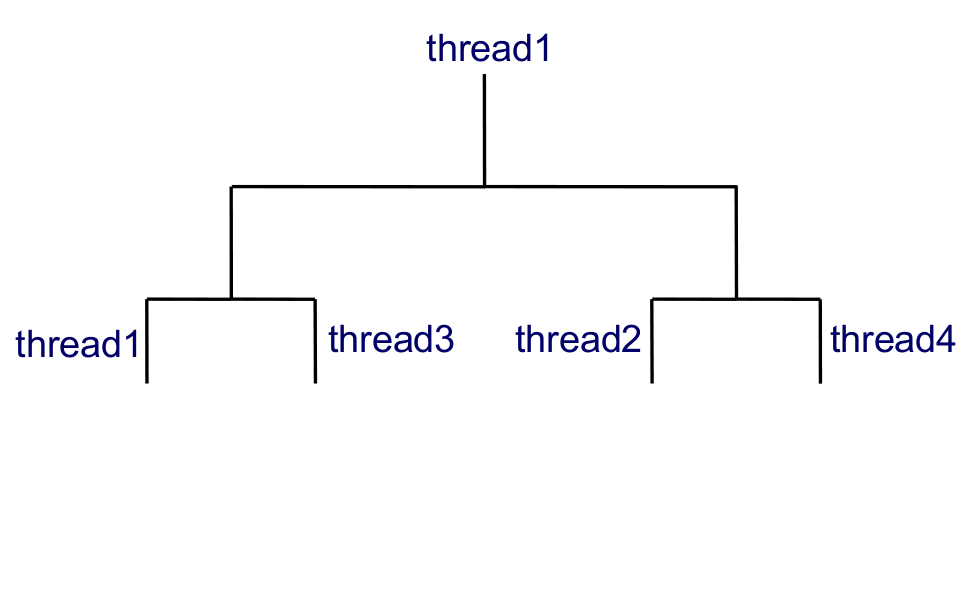
\includegraphics[width=\textwidth]{figures/thread-3}
\end{frame}

\begin{frame}{Example: Graph with 4 Threads}
  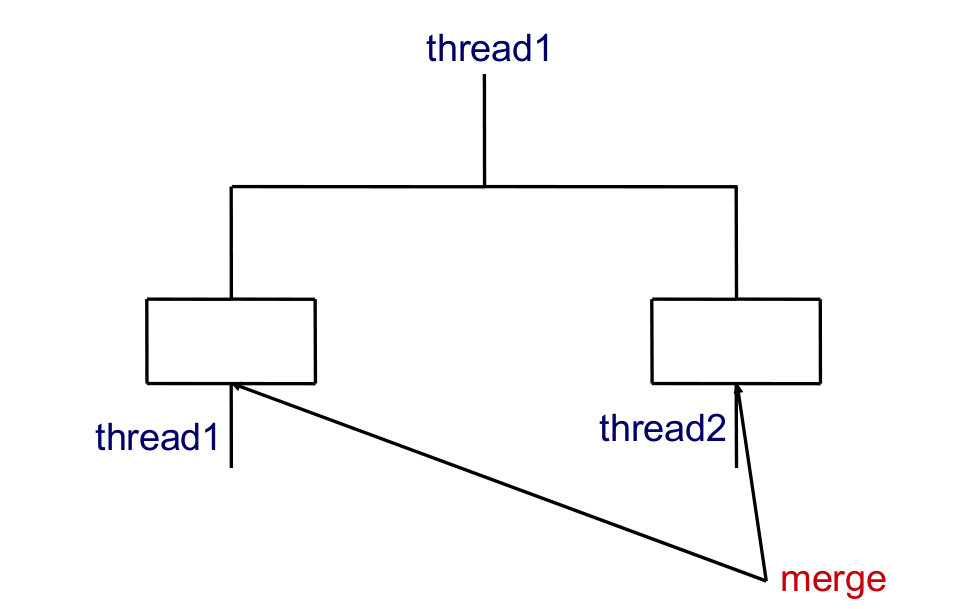
\includegraphics[width=\textwidth]{figures/thread-4}
\end{frame}

\begin{frame}{Example: Graph with 4 Threads}
  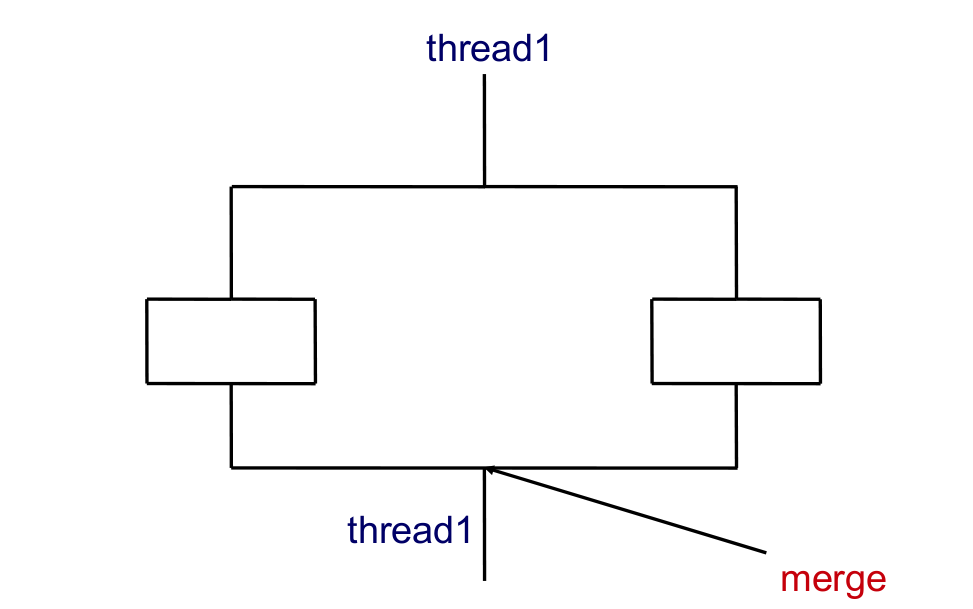
\includegraphics[width=\textwidth]{figures/thread-5}
\end{frame}

\begin{frame}{Synchronization: Join}
  \begin{itemize}
  \item \lstinline!join()! waits for this thread to die
  \item Exception: If another thread has interrupted the current
    thread
  \end{itemize}

  \vspace{\stretch{1}}

  \begin{center}
    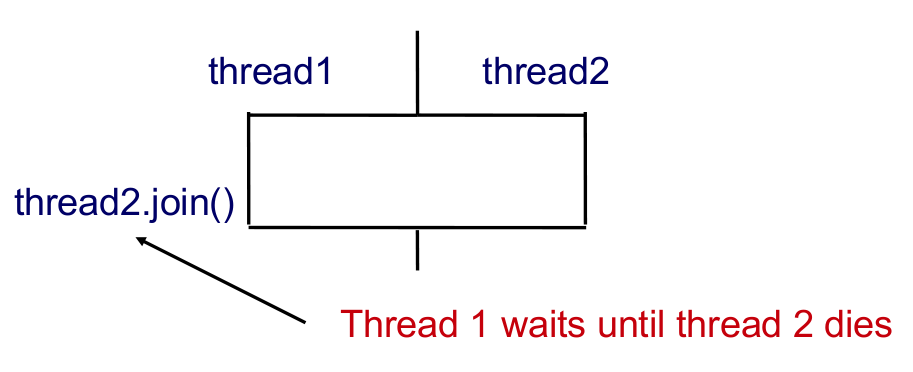
\includegraphics[scale=0.4]{figures/join}
  \end{center}
\end{frame}

\begin{frame}{Solution}
  \begin{center}
    {\huge Let's solve it together!}
  \end{center}
\end{frame}


\section{Performance Measurement}

\begin{frame}{Outline}
  \tableofcontents[current]
\end{frame}

\begin{frame}[fragile]{Measurements}
\begin{lstlisting}
int_to_sort = createRandIntArray(no_elements);
MTMergeSort m = new MTMergeSort(int_to_sort, 
                                no_threads);
// start timing
long start = System.currentTimeMillis();
m.sort();
// stop timing
long stop = System.currentTimeMillis();
long time = stop - start;
\end{lstlisting}

  \vspace{\stretch{1}}

  Extra keys for Java VM:

  \begin{itemize}
  \item \lstinline!-Xms<size>!: set initial Java heap size (eg. to
    \lstinline!1024M!)
  \item \lstinline!-Xmx<size>!: set maximum Java heap size (eg. to
    \lstinline!2048M!)
  \end{itemize}
\end{frame}

\subsection*{Results}

\begin{frame}
  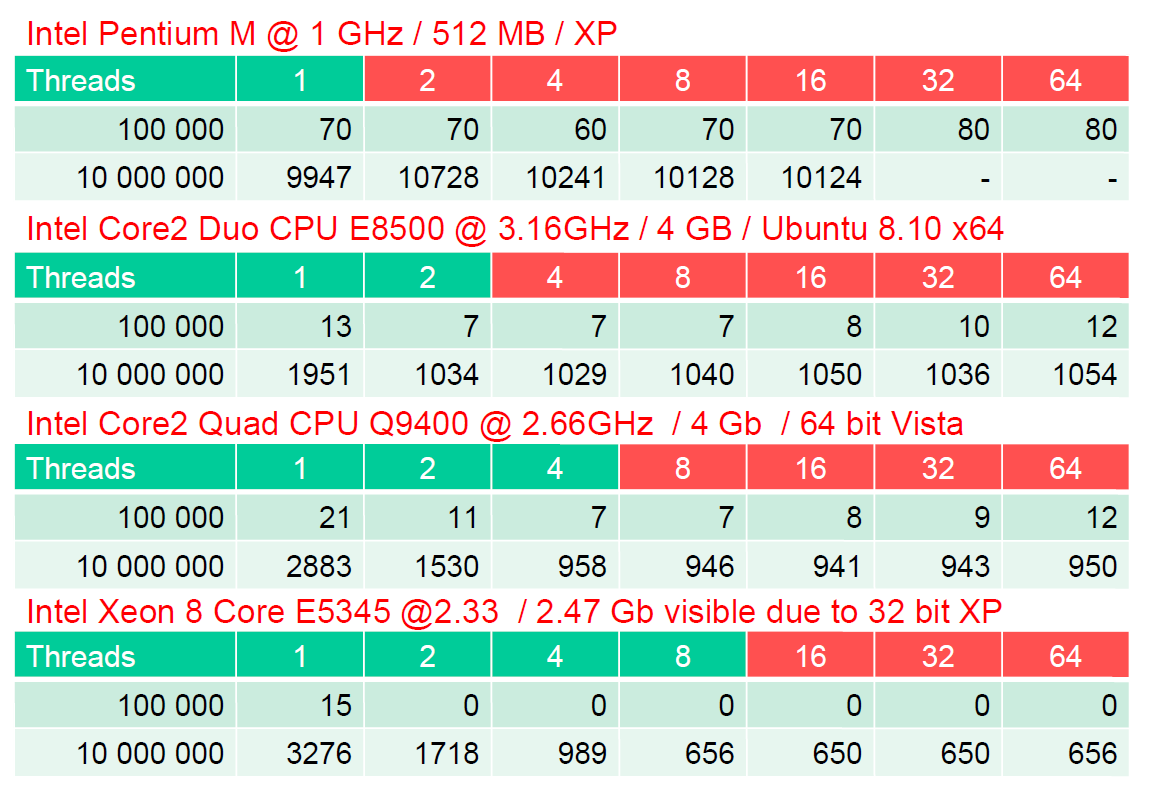
\includegraphics[width=\textwidth]{figures/measurement-1}
\end{frame}

\subsection*{Compare}

\begin{frame}
  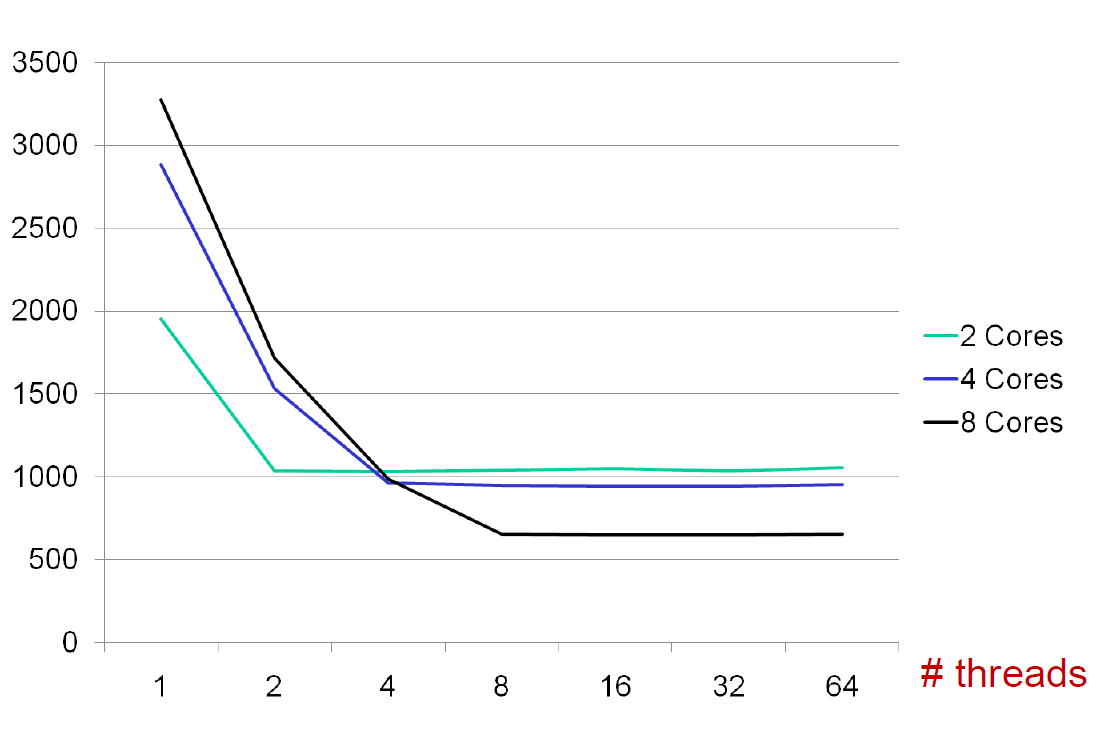
\includegraphics[width=\textwidth]{figures/measurement-2}
\end{frame}

\subsection*{More Threads}

\begin{frame}
  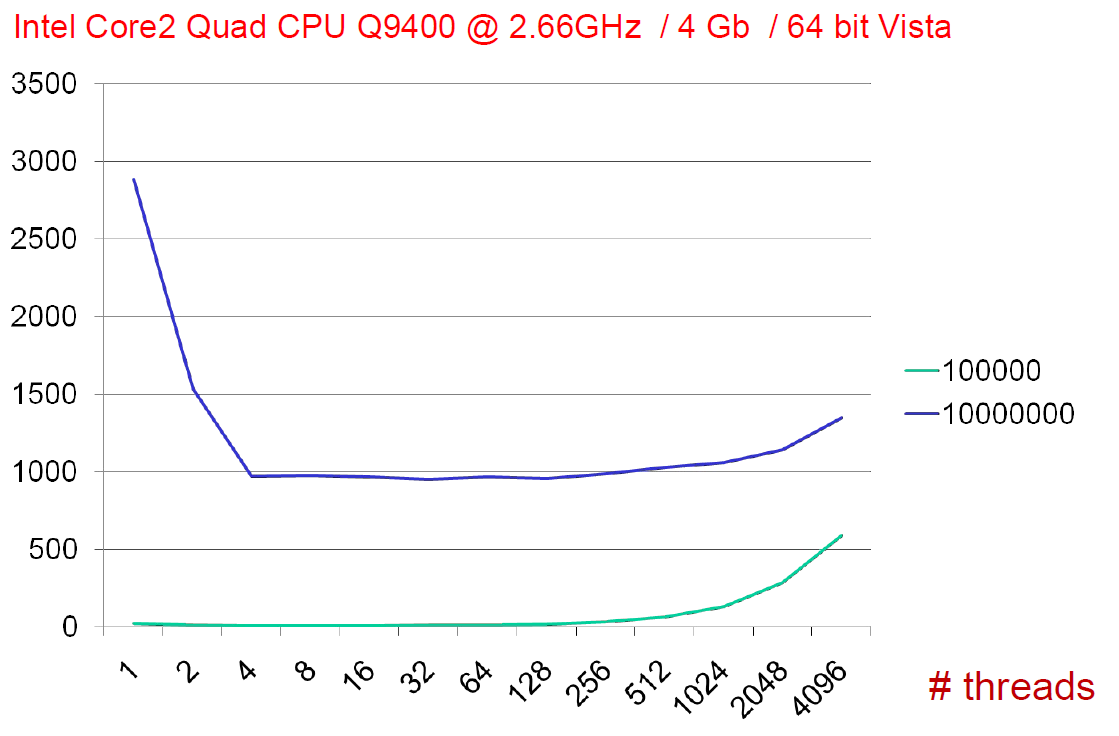
\includegraphics[width=\textwidth]{figures/measurement-3}
\end{frame}


\section{Parallel Matrix Multiplication}

\begin{frame}{Outline}
  \tableofcontents[current]
\end{frame}

\begin{frame}{Matrix Multiplication}
  \begin{itemize}
  \item Problem: Given two matrices $\mathbf{A}$, $\mathbf{B}$ of size $N \times N$.
  \item Compute the matrix product $\mathbf{C} = \mathbf{AB}$ with
    $$
    \mathbf{C}_{ij} = \sum_{k=0}^{N-1} \mathbf{A}_{ik} \cdot
    \mathbf{B}_{kj}
    $$
  \item $\mathbf{A}$, $\mathbf{B}$ elements are double-precision
    floating point numbers (\lstinline!double!)
  \end{itemize}
\end{frame}

\begin{frame}{Dense Matrices}
  \begin{itemize}
  \item Assume that $\mathbf{A}$ and $\mathbf{B}$ are dense matrices
  \item Sparse matrices have many zero elements
    \begin{itemize}
    \item Only the non-zero elements are stored
    \end{itemize}
  \item Dense matrices have mostly non-zero elements
  \item Each matrix requires $N^2$ storage cells
  \end{itemize}
\end{frame}

\begin{frame}{Parallel Matrix Multiplication}
  Which operations can be done in parallel?

 \vspace{\stretch{1}}

 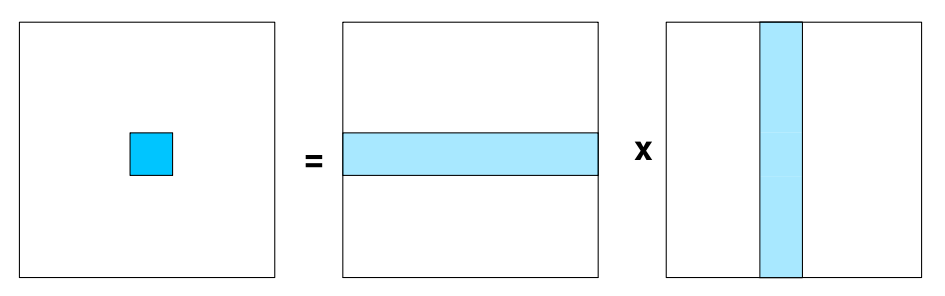
\includegraphics[width=\textwidth]{figures/matrix-1}
\end{frame}

\begin{frame}[fragile]{Programming Matrix Multiplication}
  Java code for the loop nest is easy:

\begin{lstlisting}[basicstyle=\fontsize{7}{9}\selectfont\ttfamily]
  double[][] a = new double[N][N];
  double[][] b = new double[N][N];
  double[][] c = new double[N][N];

  for (i=0; i<N; i++) {
    for (j=0; j<N; j++) {
      a[i][j] = rand.nextDouble();
      b[i][j] = rand.nextDouble();
      c[i][j] = 0.0;
    }
  }

  for (i=0; i<N; i++) {
    for (j=0; j<N; j++) {
      for (k=0; k<N; k++) {
        c[i][j] += a[i][k] * b[k][j];
      }
    }
  }
\end{lstlisting}
\end{frame}

\begin{frame}{Parallel Matrix Multiplication}
  \begin{itemize}
  \item Data partitioning based on
    \begin{itemize}
    \item Input matrix $\mathbf{A}$
    \item Input matrix $\mathbf{B}$
    \item Output matrix $\mathbf{C}$
    \end{itemize}
  \item We assume that all threads can read inputs $\mathbf{A}$ and
    $\mathbf{B}$
    \begin{itemize}
    \item Start with partitioning of output matrix $\mathbf{C}$
    \item No need to use \lstinline!synchronized!!
    \end{itemize}
  \end{itemize}
\end{frame}

\begin{frame}{Parallel Matrix Multiplication}
  Each thread computes its share of the output $\mathbf{C}$

 \vspace{\stretch{1}}

 Partition $\mathbf{C}$ by columns

 \vspace{\stretch{1}}

 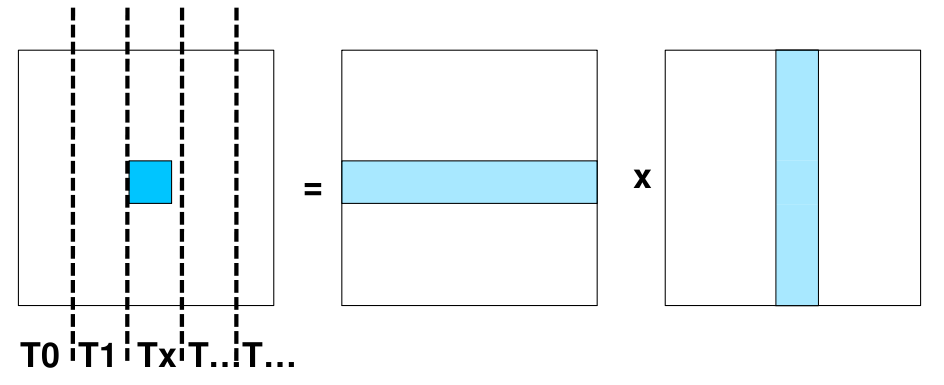
\includegraphics[width=\textwidth]{figures/matrix-2}
\end{frame}

\begin{frame}{Two Threads}
  One thread computes columns $0 \dots \frac{N}{2}$, the other columns
  $\frac{N}{2} + 1 \ldots N-1$

 \vspace{\stretch{1}}

 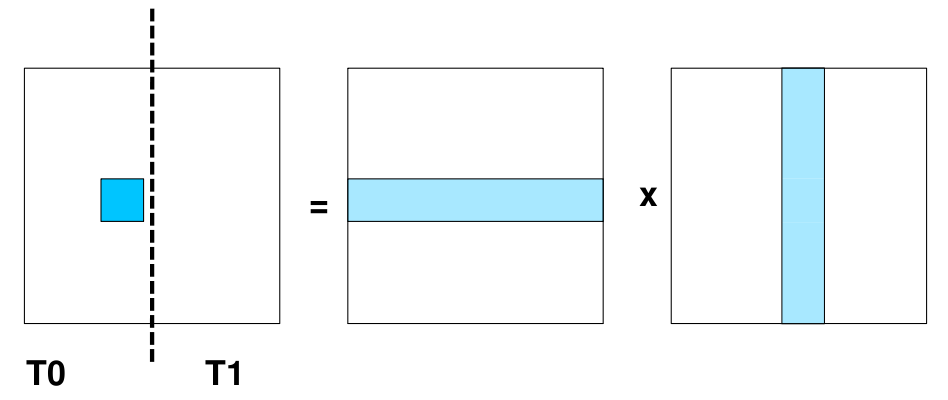
\includegraphics[width=\textwidth]{figures/matrix-3}
\end{frame}

\begin{frame}[fragile]{Two Threads}
\begin{lstlisting}
// Thread 0
for (i=0; i<N; i++) {
  for (j=0; j<N; j++) {
    for (k=0; k<N/2; k++) {
      c[i][j] += a[i][k] * b[k][j];
    }
  }
}
// Thread 1
for (i=0; i<N; i++) {
  for (j=0; j<N; j++) {
    for (k=N/2; k<N; k++) {
      c[i][j] += a[i][k] * b[k][j];
    }
  }
}
\end{lstlisting}
\end{frame}

\begin{frame}{Other Aspects}
  Partition $\mathbf{C}$ by columns or by rows?

 \vspace{\stretch{1}}

 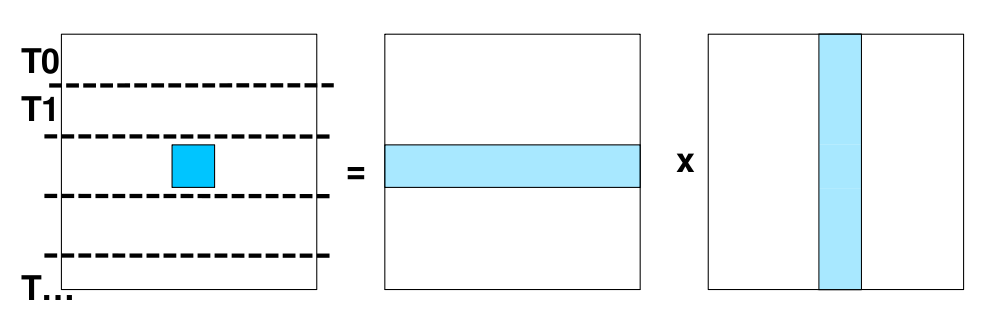
\includegraphics[width=\textwidth]{figures/matrix-4}
\end{frame}

\begin{frame}[fragile]{Other Aspects}
  What should be the order of the loops?

  \vspace{\stretch{1}}

\begin{lstlisting}
  for (i=0; i<N; i++) {
    for (j=0; j<N; j++) {
      for (k=0; k<N; k++) {
        c[i][j] += a[i][k] * b[k][j];
      }
    }
  }

  for (k=0; i<N; i++) {
    for (i=0; j<N; j++) {
      for (j=0; k<N; k++) {
        c[i][j] += a[i][k] * b[k][j];
      }
    }
  }
\end{lstlisting}
\end{frame}

\begin{frame}{Performance Measurement}
  \begin{center}
    \begin{tabular}{l||c|c|c|c|c|c|c|c|c}
      & \multicolumn{9}{c}{Number of threads} \\
      Matrix size & 1 & 2 & 4 & 8 & 16 & 32 & 64 & \ldots & 1024 \\\hline\hline
      $100$ & & & & & & & & & \\\hline
      $200$ & & & & & & & & & \\\hline
      \ldots & & & & & & & & & \\\hline
      $10'000$ & & & & & & & & & \\\hline
    \end{tabular}
  \end{center}
\end{frame}

\begin{frame}{One Thread per Matrix Element}
  \begin{center}
    {\huge Classroom exercise}
  \end{center}
\end{frame}

\begin{frame}{Don't try this at home!}
  \begin{center}
    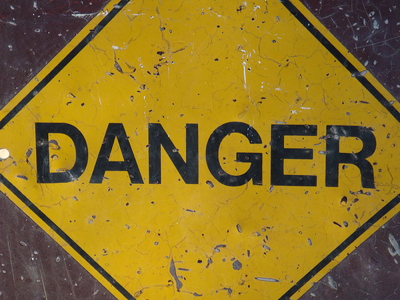
\includegraphics[scale=0.35]{figures/danger}
  \end{center}

  \vspace{\stretch{1}}

  \begin{itemize}
  \item Threads Require resources
    \begin{itemize}
    \item Memory for stacks
    \item Setup, teardown
    \end{itemize}
  \item Scheduler overhead
  \item Worse for short-lived threads
  \end{itemize}
\end{frame}


\section*{Outro}

\begin{frame}{Summary}
  \begin{itemize}
  \item Parallel MergeSort
  \item Performance issues
  \item Parallel Matrix multiplication
  \end{itemize}

  \vspace{\stretch{1}}

  \begin{center}
    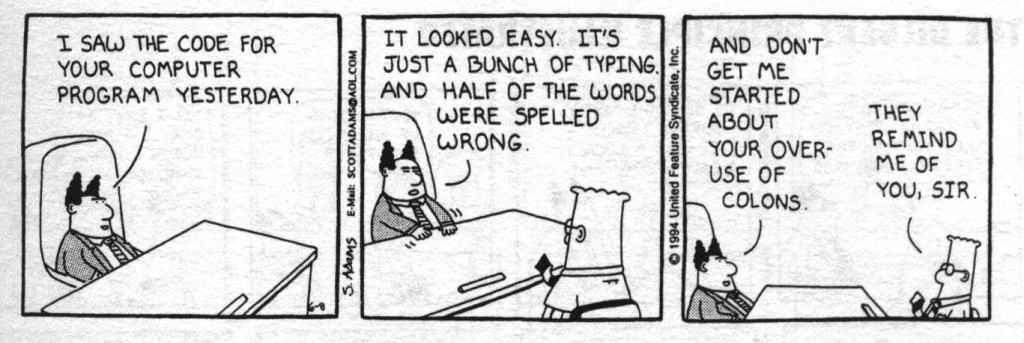
\includegraphics[scale=0.35]{figures/dilbert-2}
  \end{center}
\end{frame}

\end{document}